% !TeX spellcheck = ru_RU
% !TEX root = game_lodygin.tex

\section{Детали реализации}
В данном разделе предлагается рассмотреть основные детали реализации игровых моделей и механик. Разработка осуществлена на языке C\#.

\subsection{Концепт игры}
Действие игры происходит в недалёком прошлом, главный герой это детектив, получающий письмо с просьбой о помощи в расследовании странного дела. Игра представляет из себя последовательность локаций с возможностью их альтернативного прохождения. Игрок может пройти локацию, уничтожив всех противников в открытую, используя при этом определённый набор способностей, однако такой стиль повлияет на психическое состояние главного героя, что отразится на концовке и некоторых выборах в диалогах. С другой стороны, локацию возможно пройти скрытным путем, сохранив психическое состояние главного героя. Помимо общего психического состояния у главного героя существует динамическое состояние, на которое могут повлиять внешние факторы, например, какое-либо страшное событие, попавшее в его область видимости.

\subsection{Модель главного героя}
Модель главного героя создана с помощью программы \texttt{Fuse} от компании \texttt{Adobe}, оснащена скелетом для реализации анимирования с помощью \texttt{Mixamo} и обрезана до состояния рук с помощью программы \texttt{Blender}. Такая реализация упрощает взаимодействие с камерой, так как нет необходимости задумываться о том, что в камеру попадет внутренность головы главного героя или же предмет из рук. Для того, чтобы персонаж мог держать в руке оружие, был подключен пакет \texttt{Animation Rigging}, позволяющий на основе существующего скелета рук накладывать анимацию поверх существующих. С помощью компоненты \texttt{Two Bone IK} рука персонажа привязывается к необходимой точке, в данном случае к оружию, соблюдая при этом все костные соединения. Такая реализация позволяет в будущем иметь возможность персонажу держать не только оружие, но и любой предмет, поменяв лишь расположение костей для кисти, что упрощает взаимодействие с объектами. Из готовой модели был создан префаб для упрощения использования в различных сценах.

Модель оснащена составным коллайдером, что позволит в будущем релизовать механику ранений для разных частей тела. На данный момент имеются коллайдеры для ног, туловища, двух рук и головы.

\subsection{Передвижение игрока}
Передвижение игрока реализовано с использованием пакета \texttt{Input System}. Для считывания поступаемых данных от игрока был написан класс \texttt{InputManager}, наследуемый от главного класса \texttt{MonoBehavior}, что позволяет навесить его как компоненту на игровой объект. Далее, считываемая информация, хранящаяся в свойствах и полях данного класса, передается реализованному классу \texttt{PlayerController}, хранящему в себе реализации функций для передвижения игрока (рисунок~\ref{fig:Controller}).

\begin{figure}[H]
    \centering
    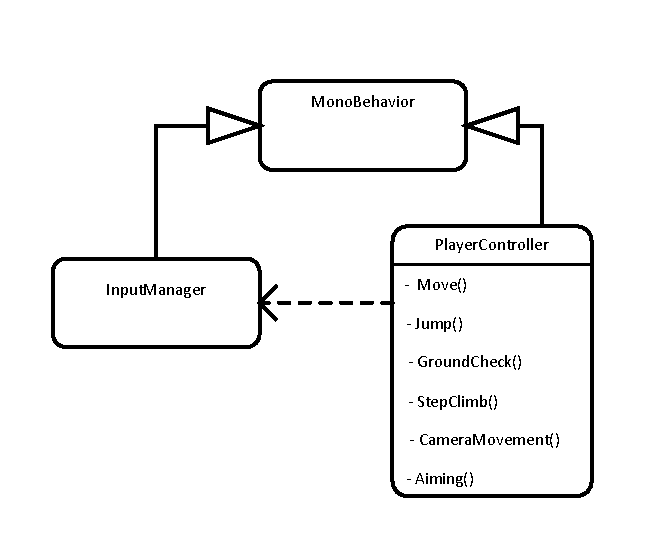
\includegraphics[width=\textwidth]{figures/PlayerController.pdf}
    \caption{Диаграмма классов для управления персонажем}
    \label{fig:Controller}
\end{figure}

Перемещение игрока реализовано с помощью применения к нему физической силы, а не изменением координат. Это позволяет иметь более плавные движения и избегать проблем с прохождением физических тел сквозь игрока, например пуль врагов. 

Для прыжка необходимо находиться на поверхности, для проверки данного состояния написана функция \texttt{GroundCheck}, которая пускает луч из центра массы тела вниз и проверяет столкновение с коллайдером поверхности.

Персонаж имеет возможность переступать через невысокие препятствия на пути, для этого написана функция \texttt{StepClimb}. Из ног и коленей персонажа пускается два луча в направлении взгляда, в случае столкновения только нижнего луча с коллайдером поверхности, персонаж перемещается прямо перед собой на высоту препятствия.
Для обзора реализована функция \texttt{CameraMovement}, принимающая значения от \texttt{InputManager} и поворачивающая камеру и физическое тело игрока на нужный угол с помощью метода \texttt{MoveRotation}.

\subsection{Оружие}
В качестве оружия реализован пистолет, на данный момент возможность стрельбы отсутствует. Модель оружия была взята из публичной библиотеки 3D моделей с соблюдением лицензии. Для управления оружием был реализован класс \texttt{WeaponController}, наследуемый от \texttt{MonoBehavior} (рисунок~\ref{fig:Weapon}). В данном классе реализованы функции для покачивания оружия в режиме <<простоя>> главного героя, для следования оружия за взглядом игрока и для тряски во время бега или ходьбы. Покачивание оружия осуществляется по траектории Лиссажу~\cite{enwiki:1187167880}.

\begin{figure}[H]
    \centering
    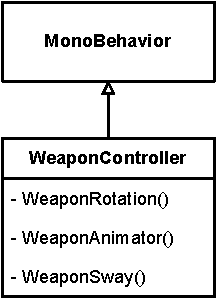
\includegraphics[width=7 cm]{figures/WeaponController.pdf}
    \caption{Диаграмма классов для оружия}
    \label{fig:Weapon}
\end{figure}

\subsection{Система психического состояния}
Для реализации динамического психического состояния главного героя был подключен пакет \texttt{PostProcessing} и реализован специальный класс \texttt{TriggerDeadBody}, наследуемый от \texttt{MonoBehavior}. Данный скрипт предназначен для ухудшения психического состояния героя при попадании в область зрения мертвого тела. При столкновении коллайдера игрока со специальным коллайдером на мертвом теле начинает осуществляться проверка нахождения мертвого тела в области видимости камеры игрока. При выполнении всех условий включается постобработка изображения игрока с постепенным усилением эффекта с течением времени.

\subsection{Система способностей}
Для реализации системы способностей создан класс \texttt{AbilityManager}, наследуемый от \texttt{MonoBehavior}. Данный класс получает информацию от класса \texttt{InputManager} и обрабатывает состояния способностей игрока. Реализован класс \texttt{Ability}, наследуемый от класса \texttt{ScriptableObject}, являющийся абстракцией над всеми способностями игрока (рисунок~\ref{fig:Ability}). Каждая способность обладает названием, активным временем и временем перезарядки, что определяет три состояния для каждой способности --- готовое, активное и перезарядка. На данный момент реализованы две способности:
\begin{enumerate}
\item  Ярость, изменяющая скорость игрока и накладывающая эффекты постобработки на изображение;
\item  Притягивание врагов. При активации способности пускается рейкаст из центра камеры игрока, в случае столкновения с коллайдером врага, враг будет притянут к игроку путем приложения к нему силы.
\end{enumerate}

\begin{figure}[H]
    \centering
    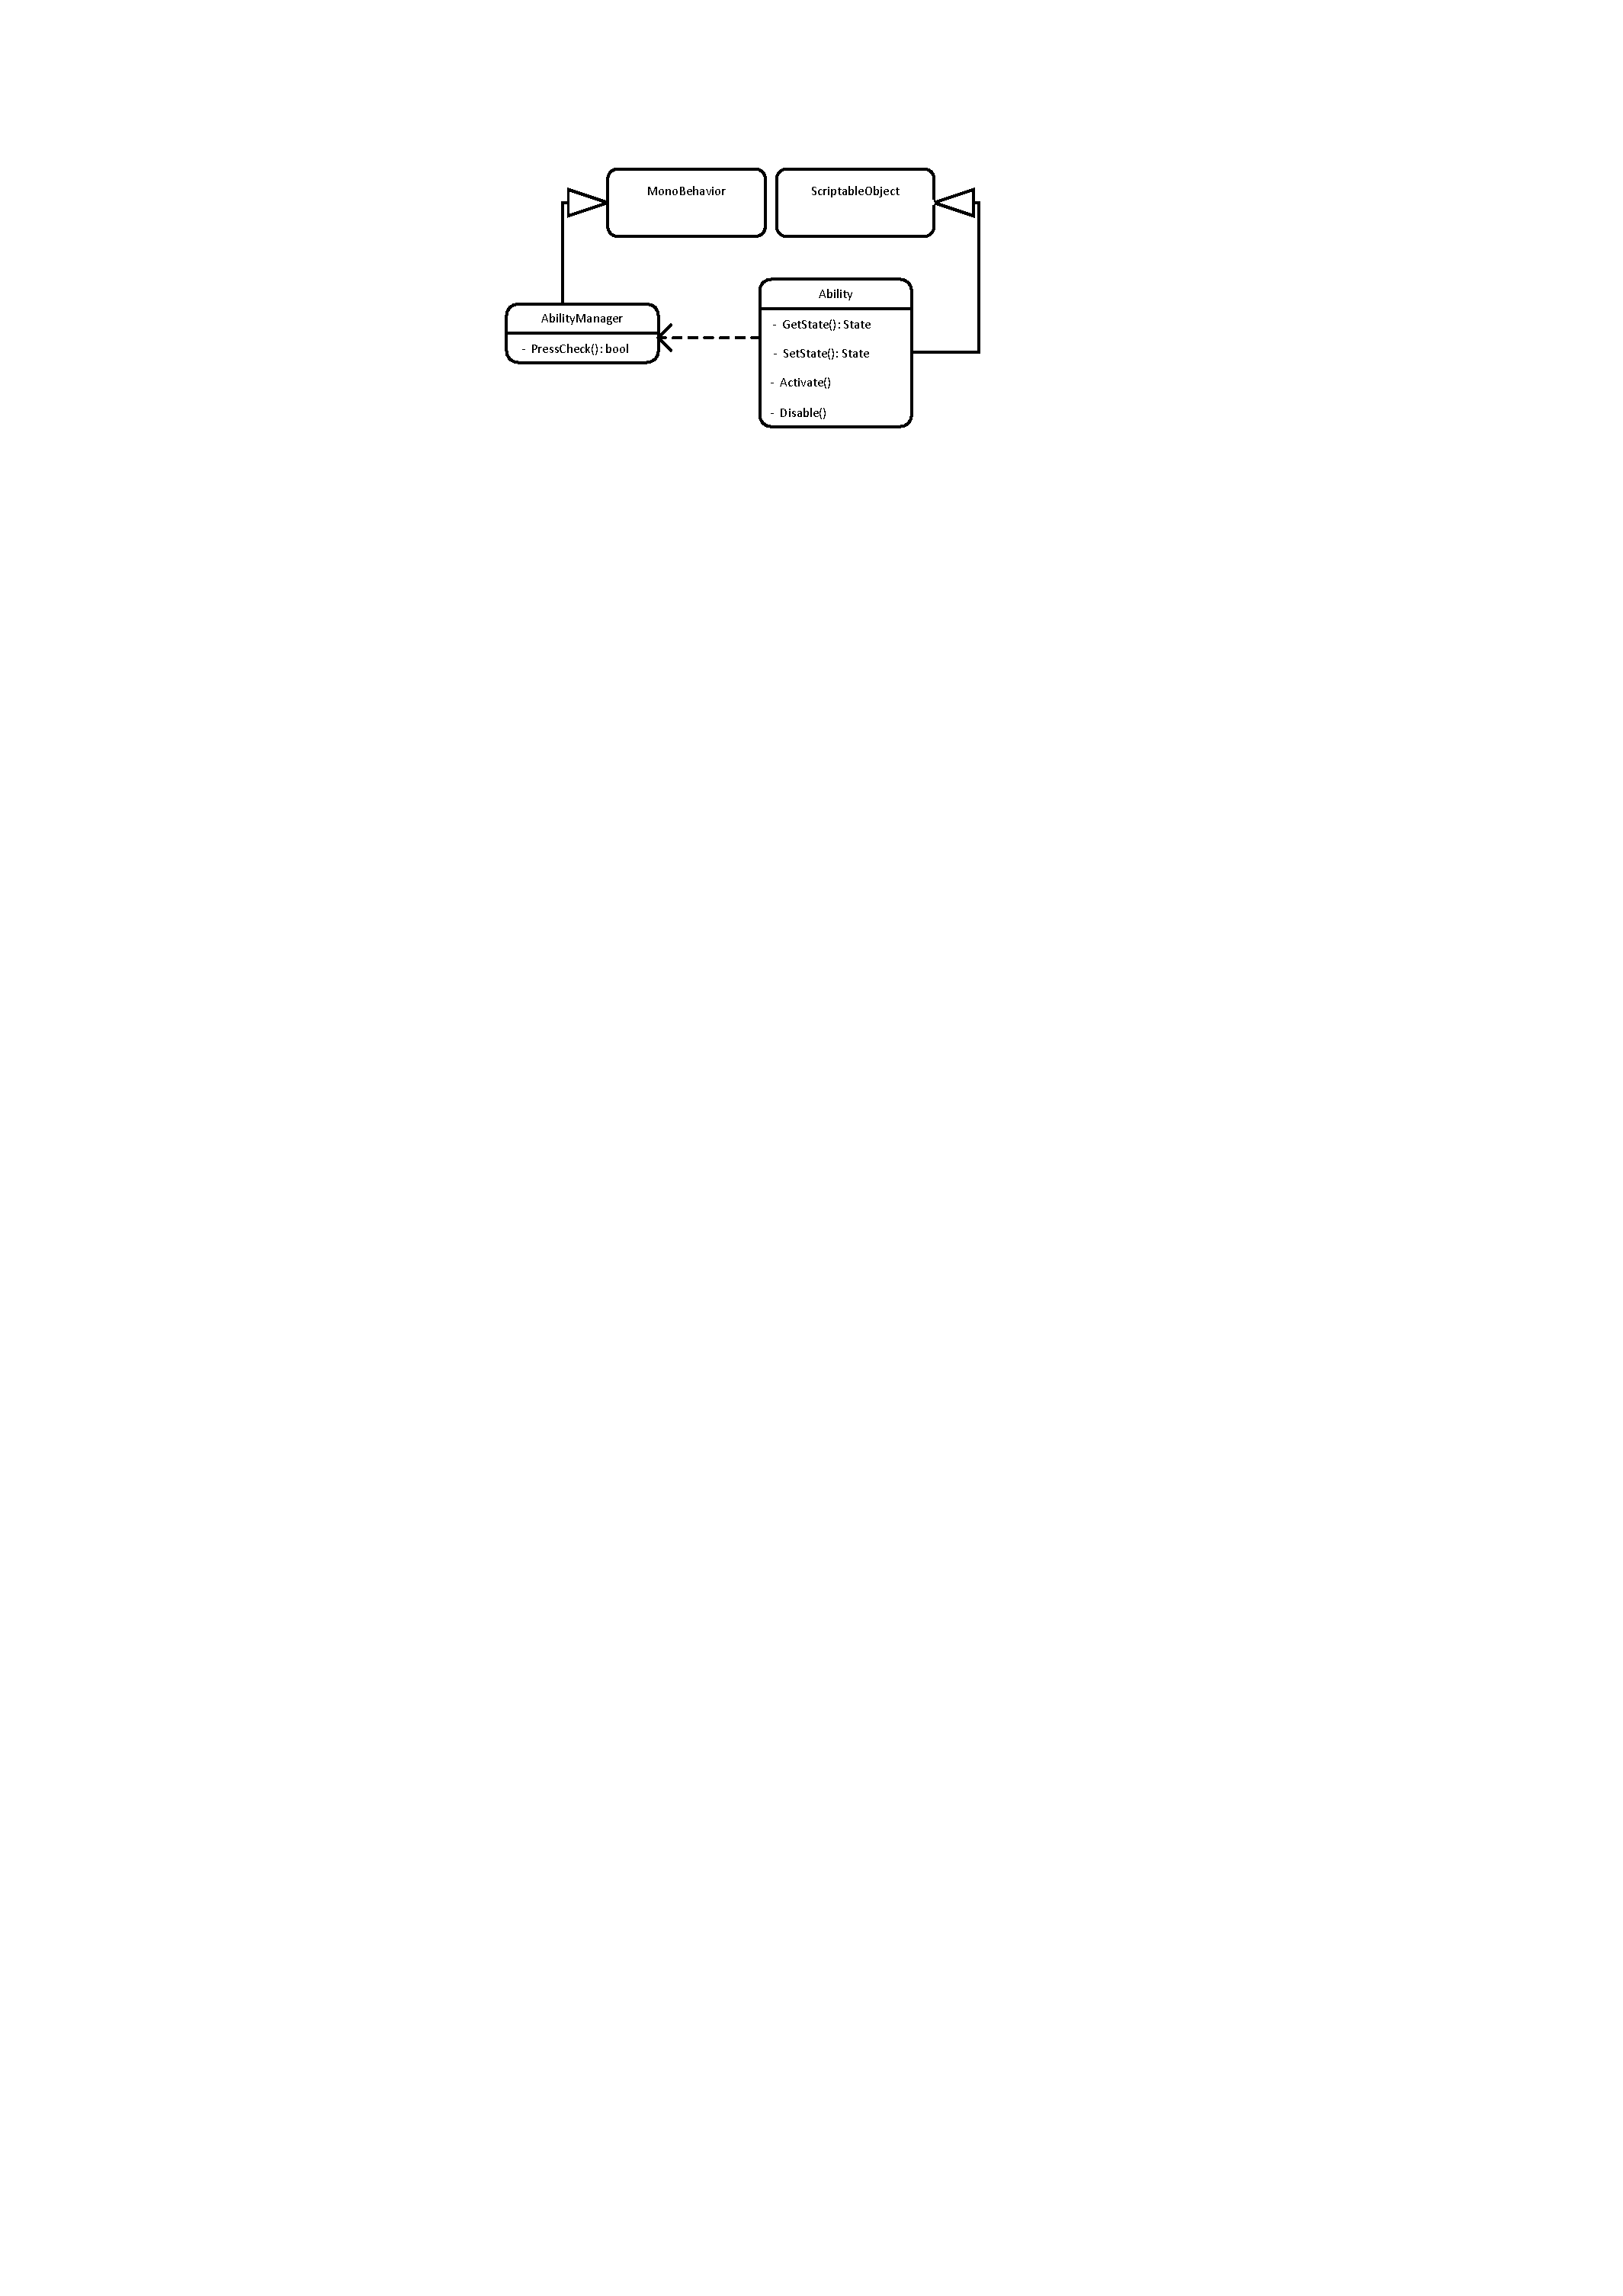
\includegraphics[width=\textwidth]{figures/Ability.pdf}
    \caption{Диаграмма классов для способностей}
    \label{fig:Ability}
\end{figure}
